% -------------------------------------------------------------------------
% Appendix: Detailed theory for empirical support seeding in MinervaRL.
% -------------------------------------------------------------------------

\section{Additional Support for MinervaRL}
\label{app:minervarl-support-bridging}

\subsection{Target-Level Reward Sparsity}
\label{app:target-level-reward-sparsity}

To characterize the sparsity that motivates hardness-gated answer-conditioned rationale generation, we analyze the
DART-CTI stage-1 plain rejection-sampling traces with a maximum budget of 32 attempts per prompt.
\Cref{fig:reward-sparsity-ate-rcm} plots target-level aggregates for ATE and RCM. Question-weighted
summaries from the target-level statistics show that ATE is sparser than RCM: ATE requires
26.7 attempts per question on average, yields 0.66 verifier-successful responses, and reaches the
32-attempt cap for 73.2\% of questions, compared with 23.6 attempts, 0.86 verifier-successful
responses, and a 61.5\% cap rate for RCM. Both tasks also exhibit long target-level tails, with many
identifiers clustered near the attempt cap and below one successful response per question.

\begin{figure}[!t]
  \centering
  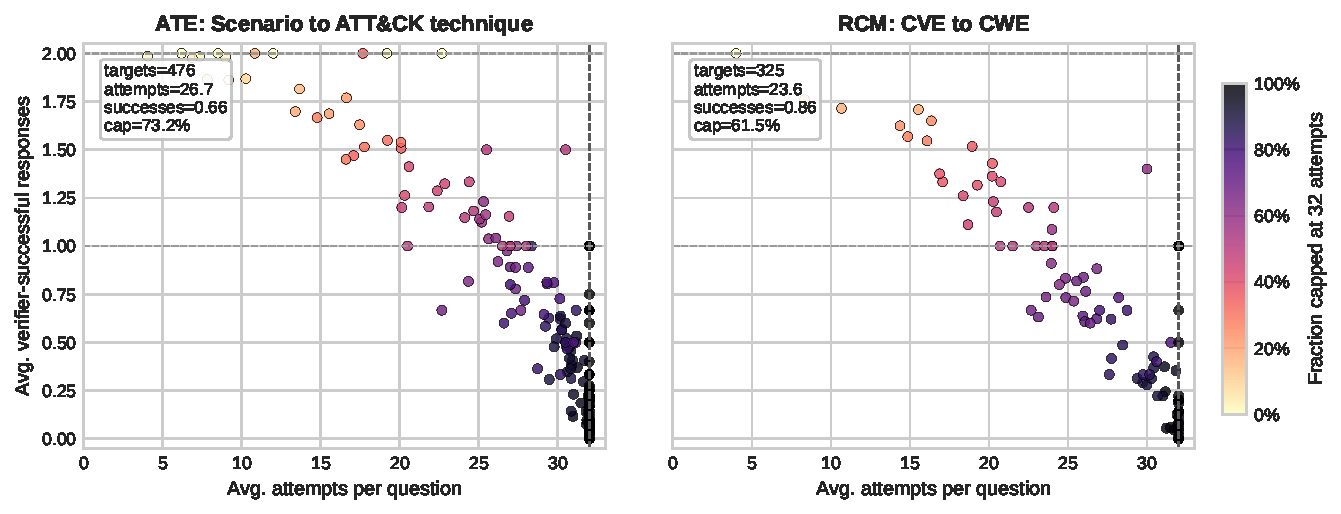
\includegraphics[width=\linewidth]{figures/reward_sparsity_ate_rcm.pdf}
  \caption{Target-level reward sparsity for ATE and RCM in DART-CTI stage-1 plain-generation attempts. Each point is one target identifier; the x-axis is mean attempts per question, the y-axis is mean verifier-successful responses per question, and color indicates the fraction of questions that reached the 32-attempt cap.}
  \label{fig:reward-sparsity-ate-rcm}
\end{figure}








% \subsection{Why MinervaRL Can Expand Empirical Support}

% \paragraph{Setup (answer-level view).}
% Each training instance is $(x, a^\star)$, where $x\in\mathcal{X}$ is the original prompt
% and $a^\star\in\mathcal{A}$ is the ground-truth structured answer
% (e.g., an ATT\&CK technique ID, a tactic set, a CVSS vector, etc.).
% Let $g:\mathcal{Y}\!\to\!\mathcal{A}$ be the task extractor mapping a full completion
% $y\in\mathcal{Y}$ to an extracted answer $a=g(y)$.

% To mirror the main text, we write the (binary) verifiable reward as
% \[
% R_{\text{minerva}}(x,y;a^\star) \;:=\; \mathbb{1}\big[g(y)=a^\star\big],
% \]
% noting that task-specific partial credit can be accommodated by thresholding at correctness.
% A policy $\pi_\theta(\cdot\mid x)$ over completions induces an \emph{answer distribution}
% \[
% p_\theta(a\mid x) \;:=\; \Pr_{y\sim \pi_\theta(\cdot\mid x)}\!\left[g(y)=a\right].
% \]
% In particular, $p_\theta(a^\star\mid x) = \Pr_{y\sim\pi_\theta}[R_{\text{minerva}}(x,y;a^\star)=1]$.

% \paragraph{Empirical support under a rollout budget.}
% Following the empirical-support viewpoint, define a detectability threshold for $k$ i.i.d.\ samples
% and failure probability $\zeta\in(0,1)$:
% \[
% \varepsilon_{k,\zeta} \;:=\; \frac{-\log \zeta}{k}.
% \]
% Intuitively, answers with probability below $\varepsilon_{k,\zeta}$ are unlikely to be observed in
% $k$ rollouts.

% \begin{lemma}[Finite-sample detectability bound]
% \label{lem:detectability}
% Fix a prompt $x$ and an answer $a\in\mathcal{A}$. Let $p=p_\theta(a\mid x)$.
% If $p \ge \varepsilon_{k,\zeta}$, then the probability that $k$ independent rollouts
% miss $a$ is at most $\zeta$:
% \[
% \Pr[\text{$a$ is not observed in $k$ rollouts}] \;=\; (1-p)^k \;\le\; \zeta.
% \]
% Equivalently, if $a$ is never observed in $k$ rollouts, then with confidence at least
% $1-\zeta$ we have $p \le \varepsilon_{k,\zeta}$.
% \end{lemma}

% \paragraph{Why small-budget RLVR can stall on ``zero-reward'' prompts.}
% Consider a training regime that (i) uses at most $k$ rollouts per prompt per iteration,
% and (ii) performs on-policy RL updates using only those sampled trajectories and their rewards.
% If $p_\theta(a^\star\mid x)\ll 1/k$, then successes on $x$ are rare; the waiting time to see the
% first success scales like $1/\text{pass@}k$.

% \begin{theorem}[Small-budget sampling barrier for on-policy RLVR (per-prompt)]
% \label{thm:rlvr-barrier}
% Fix a prompt $x$ and rollout budget $k$. Let $p_t := p_{\theta_t}(a^\star\mid x)$ be the policy's
% answer-level success probability at iteration $t$, and suppose $p_t \le \varepsilon_{k,\zeta}$.
% Then, with probability at least $1-\zeta$, the $k$ on-policy rollouts at iteration $t$ contain
% \emph{no} verified-correct trajectory for $x$. In that event, any per-prompt update rule whose
% only positive learning signal for $a^\star$ comes from \emph{observed} verified-correct rollouts
% cannot \emph{reliably} increase $p_{t+1}$ above $\varepsilon_{k,\zeta}$ in that iteration.
% \end{theorem}

% \noindent\emph{Proof sketch.}
% The first statement is \Cref{lem:detectability}.
% For the second, condition on the (typical) event that all sampled rewards are zero for prompt $x$.
% Then the update has no direct per-prompt evidence that distinguishes $a^\star$ from other
% unobserved answers under $x$ within that iteration; hence there is no reliable mechanism to move
% $p_\theta(a^\star\mid x)$ above the detectability threshold without either (a) observing a success
% for $x$, or (b) injecting an external supervised signal tied to $(x,a^\star)$.
% \hfill$\square$

% \paragraph{MinervaRL (answer-conditioned exposure + distillation).}
% MinervaRL augments RLVR with \emph{answer-conditioned rationale generation} for hard samples and
% \emph{distillation onto the original prompt}. Concretely, when $k$ base rollouts on $x$ fail,
% MinervaRL constructs a modified prompt $\tilde{x}=\mathrm{ACR}(x,a^\star,\mathrm{ref}(a^\star))$
% that reveals the gold answer $a^\star$ and (optionally) a truncated label reference. The actor samples
% $k_{\mathrm{acr}}$ completions on $\tilde{x}$, filters them using leakage/quality guards, and then performs
% SFT updates on the \emph{original} prompt $x$ using an accepted trace.

% We encode this as two assumptions: (i) answer-conditioned \emph{exposure} produces a verified trace
% with nontrivial probability, and (ii) an SFT step produces a nontrivial increase in the answer-level
% probability on the original prompt.

% \begin{assumption}[Answer-conditioned exposure for hard prompts]
% \label{ass:exposure}
% For any hard instance $(x,a^\star)$ (where base rollouts on $x$ fail),
% there exists $\alpha>0$ such that a single ACR attempt (sampling $k_{\mathrm{acr}}$ times from
% $\pi_{\theta}(\cdot\mid \tilde{x})$ and applying the MinervaRL acceptance filters) yields at least
% one accepted completion $y_{\mathrm{acr}}$ with $R_{\text{minerva}}(\tilde{x},y_{\mathrm{acr}};a^\star)=1$ with probability at least $\alpha$.
% \end{assumption}

% \begin{assumption}[Effective distillation step (answer-level)]
% \label{ass:distill}
% There exists $\Delta>0$ such that, whenever MinervaRL performs an SFT update on an accepted pair
% $(x,y_{\mathrm{acr}})$ with $R_{\text{minerva}}(x,y_{\mathrm{acr}};a^\star)=1$, the induced success probability increases by at least
% a multiplicative factor in log-space:
% \[
% \log p_{\theta^+}(a^\star\mid x) \;\ge\; \log p_{\theta}(a^\star\mid x) + \Delta,
% \]
% as long as $p_{\theta}(a^\star\mid x)$ remains below a fixed constant (i.e., before saturation).
% \end{assumption}

% \begin{theorem}[Empirical support seeding via answer-conditioned rationale distillation]
% \label{thm:minervarl-bridging}
% Fix $(x,a^\star)$ and a small rollout budget $k$ for base RLVR. Let $\varepsilon_{k,\zeta}$ be as above.
% Under \Cref{ass:exposure,ass:distill}, MinervaRL raises the success probability
% $p_\theta(a^\star\mid x)$ above the detectability threshold in a finite expected number of ACR+SFT
% cycles. In particular:
% \begin{enumerate}
% \item The number of ACR attempts until the first accepted verified trace is geometric with mean
% $\le 1/\alpha$.
% \item After $N=\left\lceil\frac{\log \varepsilon_{k,\zeta}-\log p_0}{\Delta}\right\rceil$ successful distillation
% updates on $(x,y_{\mathrm{acr}})$, we have $p_\theta(a^\star\mid x)\ge \varepsilon_{k,\zeta}$.
% \end{enumerate}
% Consequently, once $p_\theta(a^\star\mid x)\ge \varepsilon_{k,\zeta}$, the probability that the base
% RLVR rollouts on $x$ remain all-zero at budget $k$ is at most $\zeta$ (\Cref{lem:detectability}).
% \end{theorem}

% \noindent\emph{Proof sketch.}
% Item (1) is immediate from \Cref{ass:exposure}.
% Item (2) follows by iterating \Cref{ass:distill}.
% The final statement is \Cref{lem:detectability} applied to $a^\star$.
% \hfill$\square$

% \begin{corollary}[Expected cycles to cross the detectability threshold]
% \label{cor:expected-cycles}
% With the notation of \Cref{thm:minervarl-bridging}, let
% $N=\left\lceil\frac{\log \varepsilon_{k,\zeta}-\log p_0}{\Delta}\right\rceil$.
% The expected number of \emph{ACR attempts} needed to obtain $N$ successful distillation updates is at most
% $N/\alpha$ (negative-binomial), so MinervaRL crosses the detectability threshold in
% $\mathbb{E}[\text{ACR attempts}]\le N/\alpha$ under \Cref{ass:exposure,ass:distill}.
% \end{corollary}

% \paragraph{Scope and limitations.}
% The result above is intentionally narrow:
% it explains how MinervaRL can reduce the incidence of \emph{zero-reward} prompts under a \emph{fixed,
% small rollout budget} by seeding verified trajectories and distilling them onto the original prompt.
% It does \emph{not} claim that answer-conditioned rationale traces are faithful proofs, nor that the mechanism
% will transfer to domains like mathematics where conditioning on the final answer may not teach the
% model to derive it.


\subsection{Why MinervaRL Can Expand Empirical Support}
\label{app:minervarl-support-formalization}

\paragraph{Answer-level view.}
Consider a training instance $(x,a^\star)$, where $x\in\mathcal{X}$ is the original prompt and
$a^\star\in\mathcal{A}$ is the ground-truth structured answer, such as an ATT\&CK technique ID,
a set of mitigation IDs, or a CVSS vector. Let $g:\mathcal{Y}\to\mathcal{A}$ denote the
task-specific extractor that maps a full completion $y\in\mathcal{Y}$ to its final extracted answer.
For this analysis, we focus on the event of full verification and write
\begin{equation}
    S(x,y;a^\star)
    :=
    \mathbb{1}\!\left[g(y)=a^\star\right].
\end{equation}
Task-specific partial credit can be viewed as additional shaping, while the support issue studied here
concerns whether the policy samples a fully verifier-correct answer. A policy $\pi_\theta(\cdot\mid x)$
therefore induces the answer-level success probability
\begin{equation}
    p_\theta(a^\star\mid x)
    :=
    \Pr_{y\sim\pi_\theta(\cdot\mid x)}
    \left[S(x,y;a^\star)=1\right].
\end{equation}

\paragraph{Finite-budget detectability.}
With a rollout budget of $k$ independent completions for the same prompt, the probability that the
rollout group contains no fully verified completion is
\begin{equation}
    \Pr[\text{no success in $k$ rollouts}]
    =
    \left(1-p_\theta(a^\star\mid x)\right)^k .
\end{equation}
For a failure tolerance $\zeta\in(0,1)$, define the exact detectability threshold
\begin{equation}
    \varepsilon_{k,\zeta}
    :=
    1-\zeta^{1/k}
    \approx
    \frac{-\log \zeta}{k}.
\end{equation}
This is the minimum answer-level probability needed to make the chance of missing the correct answer
in $k$ samples at most $\zeta$.

\begin{lemma}[Finite-sample detectability]
\label{lem:detectability}
Fix a prompt $x$, an answer $a\in\mathcal{A}$, and a rollout budget $k$. If
$p_\theta(a\mid x)\ge \varepsilon_{k,\zeta}$, then
\begin{equation}
    \Pr[\text{$a$ is not observed in $k$ rollouts}]
    \le
    \zeta .
\end{equation}
Equivalently, observing no successful rollout is a level-$\zeta$ event under any policy that assigns
probability at least $\varepsilon_{k,\zeta}$ to the correct answer.
\end{lemma}

\noindent\emph{Proof.}
If $p_\theta(a\mid x)\ge 1-\zeta^{1/k}$, then
\[
    \Pr[\text{$a$ is not observed}]
    =
    (1-p_\theta(a\mid x))^k
    \le
    (\zeta^{1/k})^k
    =
    \zeta .
\]
\hfill$\square$

\paragraph{Small-budget all-zero regime.}
The detectability threshold above characterizes when a success is reliably observable. A stronger
``all-zero'' regime occurs when the answer probability is so small that even one success is unlikely.
For $\eta\in(0,1)$, define
\begin{equation}
    \delta_{k,\eta}
    :=
    1-(1-\eta)^{1/k}
    \approx
    \frac{\eta}{k}.
\end{equation}
If $p_\theta(a^\star\mid x)\le \delta_{k,\eta}$, then the probability of seeing no fully verified
completion in $k$ rollouts is at least $1-\eta$. Thus, when $p_\theta(a^\star\mid x)\ll 1/k$,
the prompt can repeatedly produce all-zero rollout groups.

\begin{theorem}[Small-budget support barrier for on-policy RLVR]
\label{thm:rlvr-barrier}
Fix a prompt $x$ and rollout budget $k$. Suppose that, at iteration $t$,
$p_t:=p_{\theta_t}(a^\star\mid x)\le \delta_{k,\eta}$. Then, with probability at least $1-\eta$,
the $k$ on-policy rollouts for $x$ contain no fully verified completion. On this event, any per-prompt
update rule whose direct positive signal for $a^\star$ comes only from observed verifier-correct
rollouts receives no direct evidence for increasing the probability of $a^\star$ in that iteration.
\end{theorem}

\noindent\emph{Proof sketch.}
The probability of no fully verified rollout is $(1-p_t)^k$. Since
$p_t\le 1-(1-\eta)^{1/k}$, we have $(1-p_t)^k\ge 1-\eta$. Conditioning on this event, all sampled
trajectories fail to reveal the correct answer, so an on-policy update that depends only on observed
verified successes has no per-prompt positive example of $a^\star$ to reinforce. \hfill$\square$

\paragraph{MinervaRL as support seeding.}
MinervaRL adds an auxiliary mechanism for prompts that fall into this sparse-support regime. When the
base rollouts for a prompt $x$ contain no fully verified completion, MinervaRL constructs an
answer-conditioned prompt
\[
    \tilde{x}=\mathrm{ACR}(x,a^\star,\mathrm{ref}(a^\star)),
\]
which reveals the gold answer and optionally includes a truncated canonical reference. The EMA teacher
samples ACR candidates from $\pi_\phi(\cdot\mid \tilde{x})$. A candidate is accepted only if it is
verifier-correct under the original task target and passes the leakage and quality filters. The accepted
trace is then distilled onto the original prompt $x$, not onto $\tilde{x}$.

We formalize this mechanism with two assumptions. The first states that answer-conditioned generation
can produce an accepted verified trace with nonzero probability; the second states that distilling such a
trace increases the actor's probability of producing the correct answer from the original prompt.

\begin{assumption}[Answer-conditioned exposure]
\label{ass:exposure}
For a hard instance $(x,a^\star)$, before the prompt reaches the detectability threshold
$\varepsilon_{k,\zeta}$, each ACR generation cycle has conditional probability at least $\alpha>0$
of producing an accepted trace $y_{\mathrm{acr}}$ such that
\begin{equation}
    S(x,y_{\mathrm{acr}};a^\star)=1 .
\end{equation}
\end{assumption}

\begin{assumption}[Effective original-prompt distillation]
\label{ass:distill}
Let $p_\theta(a^\star\mid x)>0$. Whenever MinervaRL performs an SFT update on an accepted pair
$(x,y_{\mathrm{acr}})$ with $S(x,y_{\mathrm{acr}};a^\star)=1$, the induced success probability under
the original prompt increases by at least $\Delta>0$ in log-space until the detectability threshold is
reached:
\begin{equation}
    \log p_{\theta^+}(a^\star\mid x)
    \ge
    \min\!\left\{
        \log \varepsilon_{k,\zeta},\,
        \log p_\theta(a^\star\mid x)+\Delta
    \right\}.
\end{equation}
\end{assumption}

\begin{theorem}[Empirical support seeding via MinervaRL]
\label{thm:minervarl-bridging}
Fix a prompt-answer pair $(x,a^\star)$, rollout budget $k$, and failure tolerance $\zeta$. Let
$\varepsilon_{k,\zeta}=1-\zeta^{1/k}$ and let
$p_0=p_{\theta_0}(a^\star\mid x)>0$. Under
Assumptions~\ref{ass:exposure} and~\ref{ass:distill}, MinervaRL raises
$p_\theta(a^\star\mid x)$ to at least $\varepsilon_{k,\zeta}$ in a finite expected number of
ACR-generation cycles. In particular, after
\begin{equation}
    L
    =
    \left\lceil
    \frac{\left[\log \varepsilon_{k,\zeta}-\log p_0\right]_+}{\Delta}
    \right\rceil
\end{equation}
successful original-prompt distillation updates, we have
\begin{equation}
    p_\theta(a^\star\mid x)\ge \varepsilon_{k,\zeta}.
\end{equation}
The expected number of ACR-generation cycles needed to obtain these $L$ accepted traces is at most
$L/\alpha$. Consequently, once this threshold is reached, the probability that standard RLVR still
misses the correct answer in $k$ rollouts is at most $\zeta$.
\end{theorem}

\noindent\emph{Proof sketch.}
By Assumption~\ref{ass:distill}, each successful distillation update increases
$\log p_\theta(a^\star\mid x)$ by at least $\Delta$ until the threshold
$\varepsilon_{k,\zeta}$ is reached. Therefore $L$ accepted distillation updates suffice. By
Assumption~\ref{ass:exposure}, each ACR-generation cycle produces an accepted trace with conditional probability
at least $\alpha$, so the expected number of cycles required to obtain $L$ accepted traces is at most
$L/\alpha$. Finally, once $p_\theta(a^\star\mid x)\ge\varepsilon_{k,\zeta}$,
Lemma~\ref{lem:detectability} implies that the probability of missing the correct answer in $k$ standard
RLVR rollouts is at most $\zeta$. \hfill$\square$

\paragraph{Scope and limitations.}
This argument is intentionally narrow. It explains how MinervaRL can reduce the incidence of
zero-success rollout groups under a fixed, small rollout budget by seeding verified traces and distilling
them onto the original prompt. It does not claim that ACR traces are faithful proofs, that every accepted
trace improves general reasoning, or that answer conditioning is sufficient in domains where knowing the
final answer does not help construct a valid derivation.
